\documentclass[11pt, a4paper]{article}

\usepackage[margin=2.5cm]{geometry}
\usepackage{graphicx}
\usepackage{booktabs}
\usepackage{hyperref}

\title{Transcriptome Changes Caused by Deletion of \textit{MIG1} in \textit{Saccharomyces cerevisiae}: A Re-analysis of Public RNA-seq Data (GSE104356)}
\author{Ajay Nath}
\date{\today}

\begin{document}

% --- Page 1: title page ---
\begin{titlepage}
\centering
\vspace*{3cm}
{\LARGE\bfseries Transcriptome Changes Caused by Deletion of \textit{MIG1} in \textit{Saccharomyces cerevisiae}\par}
\vspace{0.8cm}
{\Large A Re-analysis of Public RNA-seq Data (GSE104356)\par}
\vspace{3cm}
{\large Ajay Nath\par}
\vspace{0.5cm}
{\large \today\par}
\vfill
{\normalsize RNA-seq analysis: FastQC, fastp, STAR, featureCounts, DESeq2, clusterProfiler\par}
\end{titlepage}

% --- Page 2: table of contents ---
\tableofcontents
\clearpage

% --- Page 3: abstract and the rest ---
\section*{Abstract}
\addcontentsline{toc}{section}{Abstract}
Mig1 is the main DNA-binding repressor of glucose-repressed genes in \textit{Saccharomyces cerevisiae}. We re-analysed public paired-end RNA-seq data (GEO GSE104356) comparing a \textit{mig1}$\Delta$ strain with its wild type (WT), two samples each, grown at 40$^\circ$C. Reads were quality-checked, trimmed, aligned to the R64-1-1 genome, counted per gene and tested with DESeq2. Of 5,969 tested genes, 389 changed significantly in the deletion strain (193 up, 196 down; adjusted $p<0.05$, $|\log_2\mathrm{FC}|>1$). \textit{MIG1} itself fell about 150-fold, and the classic glucose-repressed genes \textit{HXK1} and \textit{HXT2} rose. Up-regulated genes were enriched for metal ion and sugar transport, cell wall and vacuole, and the pheromone response, while ER protein-folding genes were down-regulated. One KO library (SRR6108784) was contaminated with \textit{Drosophila} RNA and primer concatemers, leaving about 3 million usable read pairs. With two samples per group, the findings are hypothesis-generating.

\noindent\textbf{Keywords:} \textit{Saccharomyces cerevisiae}, MIG1, RNA-seq, differential expression, DESeq2, Gene Ontology

\section{Introduction}
In the presence of glucose, yeast represses the genes needed to use alternative carbon sources. The zinc-finger protein Mig1 is the central DNA-binding repressor of this carbon catabolite repression \cite{nehlin1990,gancedo1998}. Deleting \textit{MIG1} is therefore expected to release glucose-repressed genes, but the wider transcriptional consequences under stress are less clear.

GEO series GSE104356 profiles a wild-type strain (ScY01a) and four transcription factor deletions (\textit{ric1}$\Delta$, \textit{srb2}$\Delta$, \textit{sin3}$\Delta$, \textit{mig1}$\Delta$) grown at 40$^\circ$C, a condition used to study long-term thermal stress tolerance \cite{edgar2002}. Here we use only the WT and \textit{mig1}$\Delta$ samples and ask: (i) which genes change when \textit{MIG1} is deleted, (ii) whether known Mig1 targets behave as expected, and (iii) which biological processes are affected. We also document the quality problems found in the public data and how they were handled.

\section{Materials and Methods}

\subsection{Data}
Run information was retrieved from the European Nucleotide Archive (BioProject PRJNA412405) \cite{leinonen2011}. The data are 151\,bp paired-end Illumina HiSeq 4000 reads. We analysed two WT runs (SRR6108775, SRR6108776) and two \textit{mig1}$\Delta$ (KO) runs (SRR6108783, SRR6108784). Both runs of a strain share one GEO sample, so we could not verify from the database that they are independent cultures. FASTQ files were downloaded over https, http or ftp, whichever the server offered, and accepted only when the file size matched the ENA value. Integrity was checked with a gzip test and by comparing read counts with ENA.

\subsection{Quality control and trimming}
Raw and trimmed reads were assessed with FastQC \cite{andrews2010} and summarised with MultiQC \cite{ewels2016}. Adapters were detected automatically and removed with fastp \cite{chen2018}, with a minimum read length of 36. PCR duplicates were not removed, because high duplication is expected in RNA-seq.

\subsection{Alignment and counting}
Reads were aligned with STAR 2.7.10b \cite{dobin2013} to the \textit{S. cerevisiae} R64-1-1 genome with the Ensembl Genomes fungi release 56 annotation. The index used \texttt{sjdbOverhang} 150 and \texttt{genomeSAindexNbases} 10. Maximum intron length and mate gap were set to 2,000\,bp. Library strandedness was tested on all four samples with featureCounts; all libraries were unstranded (about 81--84\% of pairs assigned with \texttt{-s 0}, about 46\% with \texttt{-s 1} or \texttt{-s 2}). Read pairs were counted per gene on exons with featureCounts v2.1.1 \cite{liao2014}, using \texttt{-s 0}. Multi-mapping pairs were not counted.

\subsection{Differential expression}
Analysis used DESeq2 1.50.2 \cite{love2014} in R, with the design \texttt{\textasciitilde\,condition} and WT as reference. Genes with at least 10 reads in at least two samples were kept. Size factors, dispersions and Wald tests were computed with \texttt{DESeq()}. Fold changes were shrunk with apeglm \cite{zhu2019}. $p$-values were adjusted by the Benjamini--Hochberg method \cite{benjamini1995}. A gene was called significant at adjusted $p<0.05$ and shrunken $|\log_2\mathrm{FC}|>1$. As a consistency check, we required both KO samples to lie on the same side of both WT samples after normalisation.

\subsection{Functional enrichment}
Gene Ontology \cite{ashburner2000} enrichment (Biological Process, Molecular Function, Cellular Component) was run separately for up- and down-regulated genes with clusterProfiler \cite{wu2021} and the \texttt{org.Sc.sgd.db} annotation \cite{cherry2012}. The background was all tested genes, and terms were kept at Benjamini--Hochberg adjusted $p<0.05$.

\section{Results}

\subsection{Data quality}
Raw FastQC showed per-base quality mostly above Q30, a normal composition bias in the first 15 bases, and trace adapter content. After fastp trimming, adapter content passed in all files and mates stayed in sync (Table~\ref{tab:trim}). fastp detected TruSeq adapters in three samples but Nextera adapters in SRR6108784, which also had shorter inserts (about 169\,bp), higher GC (46\% versus 40--41\%) and reads that were repeats of a SMART-type primer sequence. KO replicates therefore come from different library preparations.

\begin{table}[ht]
\centering
\caption{Trimming and alignment summary.}
\label{tab:trim}
\begin{tabular}{llrrrr}
\toprule
Run & Group & Pairs kept & Unique (\%) & Multi (\%) & Too short (\%) \\
\midrule
SRR6108775 & WT & 8,029,008 & 93.46 & 4.50 & 1.88 \\
SRR6108776 & WT & 7,284,012 & 93.84 & 4.14 & 1.88 \\
SRR6108783 & KO & 8,040,003 & 92.65 & 4.73 & 2.44 \\
SRR6108784 & KO & 8,657,664 & 36.54 & 1.72 & 61.68 \\
\bottomrule
\end{tabular}
\end{table}

\subsection{Contamination in SRR6108784}
Only 36.5\% of SRR6108784 pairs mapped uniquely, and 61.7\% were unmapped as ``too short''. Relaxing the STAR filters raised unique mapping only to 40.6\%, so most unmapped pairs are not yeast. BLAST of ten random non-primer unmapped reads gave \textit{Drosophila melanogaster} as the top hit for all ten, and about 20\% of unmapped pairs carried the primer motif. Unmapped reads had 49\% GC, against about 40\% for yeast. The yeast part of the library behaved normally (83.6\% of mapped pairs assigned to genes, as in the other samples), and about 3.0 million assigned pairs remained, against 6.3--7.0 million for the others. We kept the sample, since each group has only two.

\subsection{Sample-level structure}
After filtering, 6,291 genes passed a total-count filter, and 5,969 passed the final filter. In a PCA of the 500 most variable genes, PC1 (83.7\% of variance) separated WT from KO, with SRR6108784 next to SRR6108783. PC2 (9.8\%) separated first from second replicates in both groups, so it is not specific to the contaminated library. WT replicates differed more than KO replicates.

\subsection{Differential expression}
DESeq2 size factors were 1.23--1.27 for three samples and 0.53 for SRR6108784, in line with its lower depth. At adjusted $p<0.05$, 299 genes were up and 340 down in KO; with the additional $|\log_2\mathrm{FC}|>1$ cutoff, 193 were up and 196 down (Figure~\ref{fig:volcano}). Of the 389 genes, 370 are protein-coding. Every one of them showed both KO samples on the same side of both WT samples.

\textit{MIG1} (YGL035C) fell from 321 and 576 reads in WT to 4 and 0 in KO ($\log_2\mathrm{FC}=-7.2$, adjusted $p=2\times10^{-16}$), confirming the deletion. Known glucose-repressed genes moved as expected: \textit{HXT2} rose about 6.6-fold and \textit{HXK1} about 16-fold, and \textit{SUC2} rose 1.7-fold (significant, but below the 2-fold cutoff). The \textit{GAL} genes were unchanged. The strongest increases included the iron uptake genes \textit{FIT1}, \textit{FIT3}, \textit{FET3} and \textit{SIT1}, the copper transporter \textit{CTR3} and the phosphate transporter \textit{PHO84}. The strongest decreases outside \textit{MIG1} included \textit{INO1} and the ER chaperone \textit{KAR2}.

\begin{figure}[ht]
\centering
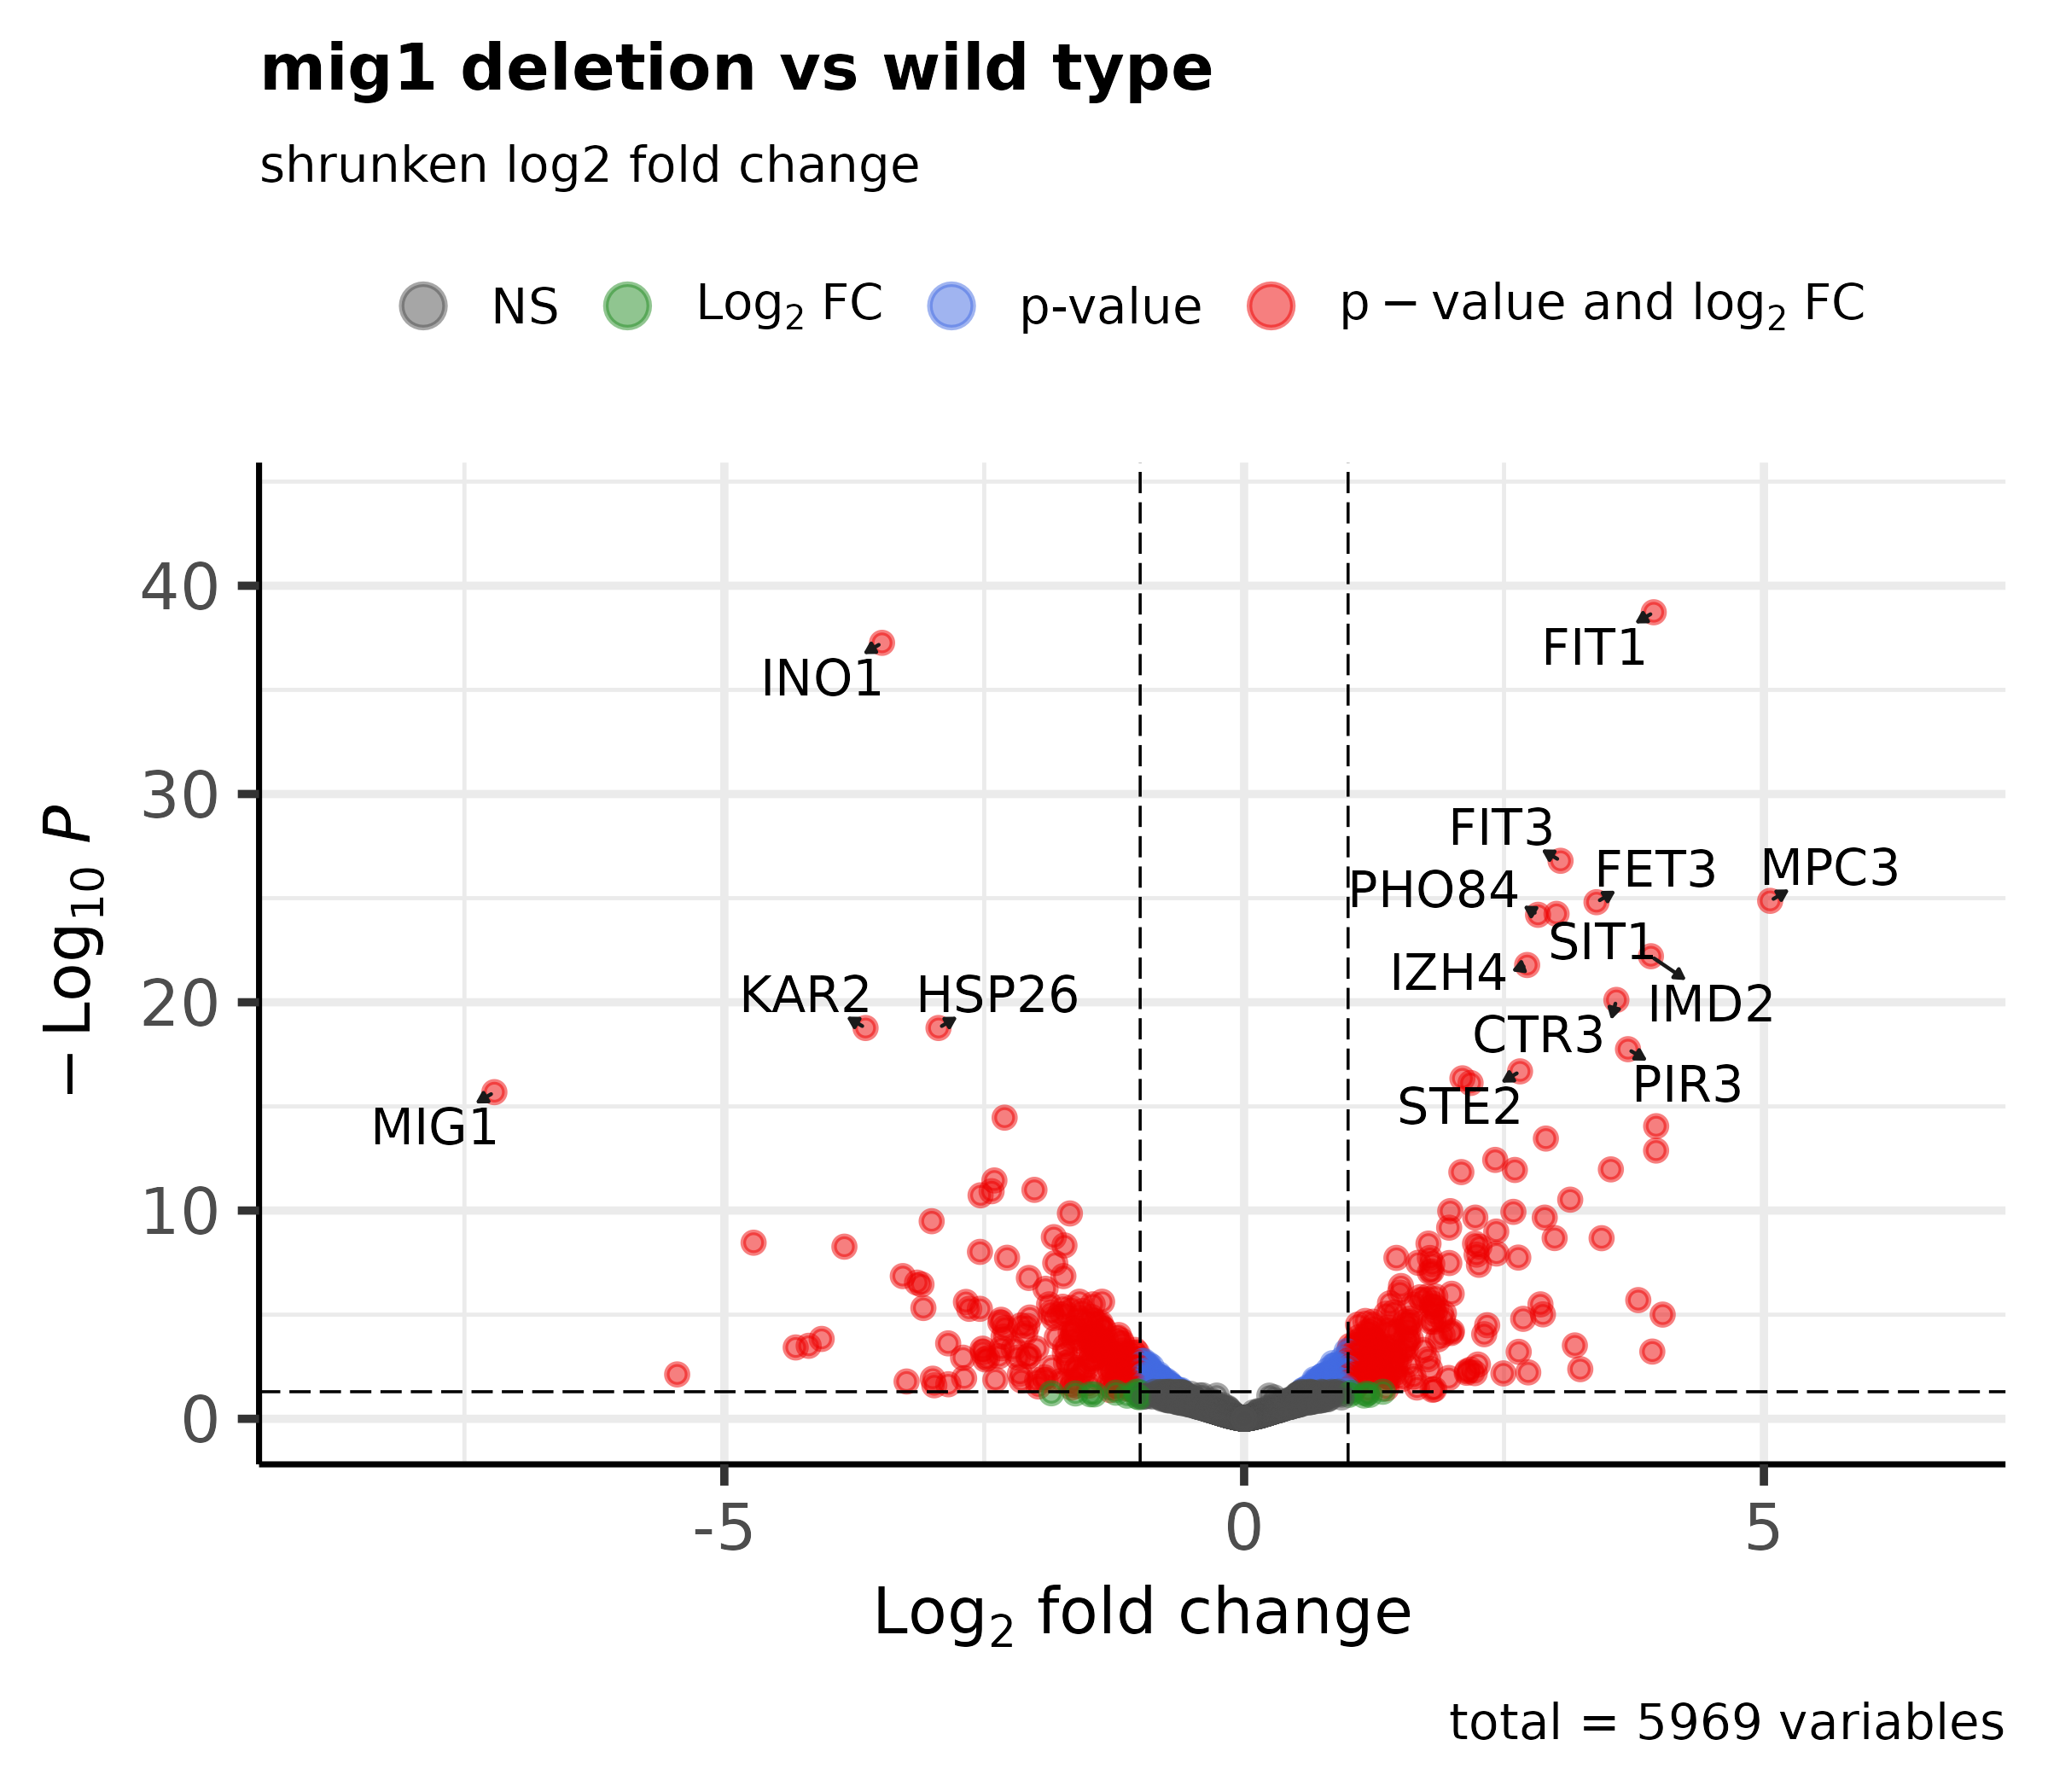
\includegraphics[width=0.85\textwidth]{../results/deseq2/volcano.png}
\caption{Volcano plot of \textit{mig1}$\Delta$ versus wild type (shrunken $\log_2$ fold change against $-\log_{10}$ adjusted $p$). Cutoffs: adjusted $p=0.05$ and $|\log_2\mathrm{FC}|=1$.}
\label{fig:volcano}
\end{figure}

\subsection{Functional enrichment}
Up-regulated genes gave 75 Biological Process terms, led by metal ion transport (transition metal ion transport, 20 of 190 genes, adjusted $p=3\times10^{-11}$; iron and copper transport), then sugar transport, central carbon metabolism, mating and pheromone response, and cell wall organisation. Molecular Function and Cellular Component agreed (transporter activity; cell wall, fungal-type vacuole, mating projection). Down-regulated genes gave 3 Biological Process terms (protein folding, response to ER stress, protein maturation; adjusted $p=0.004$--$0.014$), with unfolded protein binding, disulfide oxidoreductase activity and the ER lumen in the other ontologies.

\section{Discussion}
The deletion was clearly detected, and glucose-repressed genes such as \textit{HXK1} and \textit{HXT2} were derepressed, consistent with the known role of Mig1 \cite{nehlin1990,gancedo1998}. The up-regulation of sugar transporters and carbon metabolism fits this role. The strong metal uptake signature (iron, copper) is less obvious. It resembles a starvation-type response, but Mig1 is not a known regulator of iron genes, so the link may be indirect or may reflect a difference in culture state. Likewise, the lower expression of the ER folding machinery suggests reduced ER stress in the KO, but these data cannot give a mechanism.

The up-regulated pheromone-pathway genes (\textit{STE2}, \textit{BAR1}, \textit{AGA1}, \textit{AGA2}) were unexpected. A mating-type difference between the strains was considered, but reads at the silent \textit{HMRA1} locus appeared in all four samples and \textit{MATALPHA1} was essentially absent, so both strains appear to be MATa. The cause remains unexplained, and we report it as an observation only.

\section{Limitations}
\begin{itemize}
  \item Two samples per group give low power, so results are hypothesis-generating.
  \item Both runs of a strain share one GEO sample, so independence of replicates is unproven. The KO replicates were prepared with different library methods (TruSeq and Nextera), which cannot be corrected for with $n=2$.
  \item SRR6108784 is contaminated with \textit{Drosophila} RNA and primer dimers, giving lower depth and noisier low-count genes. A competitive alignment to a combined yeast and fly genome was not done.
  \item Growth conditions (glucose level, temperature) and whether WT and KO share the same genetic background were not confirmed from the source publication.
  \item snoRNA and tRNA hits (about 13 genes) are unreliable, because poly(A) selection captures them poorly.
  \item GSEA and KEGG analyses were not performed.
\end{itemize}

\section{Conclusion}
Deleting \textit{MIG1} changed the expression of 389 of 5,969 tested genes. The deletion and known glucose-repressed targets behaved as expected, and the data suggest changes in metal and sugar transport, cell wall and vacuole, the pheromone response and ER protein folding. Because of the small sample size and one contaminated library, these patterns need independent validation.

\section*{Data and Code Availability}
\addcontentsline{toc}{section}{Data and Code Availability}
Raw data: GEO GSE104356, ENA/BioProject PRJNA412405 (SRA SRP119006). The analysis was done with a conda environment (STAR, featureCounts, fastp, FastQC, MultiQC, R/DESeq2) and an R Markdown notebook kept in the project repository.

\addcontentsline{toc}{section}{References}
\begin{thebibliography}{99}

\bibitem{andrews2010} Andrews S. FastQC: a quality control tool for high throughput sequence data. Babraham Bioinformatics, 2010.

\bibitem{ashburner2000} Ashburner M, et al. Gene Ontology: tool for the unification of biology. \textit{Nature Genetics} 25:25--29, 2000.

\bibitem{benjamini1995} Benjamini Y, Hochberg Y. Controlling the false discovery rate: a practical and powerful approach to multiple testing. \textit{Journal of the Royal Statistical Society B} 57:289--300, 1995.

\bibitem{chen2018} Chen S, Zhou Y, Chen Y, Gu J. fastp: an ultra-fast all-in-one FASTQ preprocessor. \textit{Bioinformatics} 34:i884--i890, 2018.

\bibitem{cherry2012} Cherry JM, et al. Saccharomyces Genome Database: the genomics resource of budding yeast. \textit{Nucleic Acids Research} 40:D700--D705, 2012.

\bibitem{dobin2013} Dobin A, et al. STAR: ultrafast universal RNA-seq aligner. \textit{Bioinformatics} 29:15--21, 2013.

\bibitem{edgar2002} Edgar R, Domrachev M, Lash AE. Gene Expression Omnibus: NCBI gene expression and hybridization array data repository. \textit{Nucleic Acids Research} 30:207--210, 2002.

\bibitem{ewels2016} Ewels P, Magnusson M, Lundin S, K{\"a}ller M. MultiQC: summarize analysis results for multiple tools and samples in a single report. \textit{Bioinformatics} 32:3047--3048, 2016.

\bibitem{gancedo1998} Gancedo JM. Yeast carbon catabolite repression. \textit{Microbiology and Molecular Biology Reviews} 62:334--361, 1998.

\bibitem{leinonen2011} Leinonen R, et al. The European Nucleotide Archive. \textit{Nucleic Acids Research} 39:D28--D31, 2011.

\bibitem{liao2014} Liao Y, Smyth GK, Shi W. featureCounts: an efficient general purpose program for assigning sequence reads to genomic features. \textit{Bioinformatics} 30:923--930, 2014.

\bibitem{love2014} Love MI, Huber W, Anders S. Moderated estimation of fold change and dispersion for RNA-seq data with DESeq2. \textit{Genome Biology} 15:550, 2014.

\bibitem{nehlin1990} Nehlin JO, Ronne H. Yeast MIG1 repressor is related to the mammalian early growth response and Wilms' tumour finger proteins. \textit{EMBO Journal} 9:2891--2898, 1990.

\bibitem{wu2021} Wu T, et al. clusterProfiler 4.0: a universal enrichment tool for interpreting omics data. \textit{The Innovation} 2:100141, 2021.

\bibitem{zhu2019} Zhu A, Ibrahim JG, Love MI. Heavy-tailed prior distributions for sequence count data: removing the noise and preserving large differences. \textit{Bioinformatics} 35:2084--2092, 2019.

\end{thebibliography}

\end{document}
